\documentclass[aspectratio=169]{beamer}
\usepackage[utf8]{inputenc}
\usepackage{lmodern}
\usepackage{utopia} % font utopia imported

\usetheme{Madrid}
\usecolortheme{beaver}


\usepackage{textpos}
\usepackage{animate}

\usepackage{graphicx}

\usepackage{commath}

\setbeamertemplate{caption}[numbered]

\usepackage{fvextra}

% Includes "References" in the table of contents

\usepackage[nottoc]{tocbibind}
\usepackage[autostyle = true]{csquotes}

\usepackage[backend=biber,style=ieee]{biblatex}
\urlstyle{same}
\addbibresource{bibliography.bib}

% Hyperlinks settings

\usepackage{hyperref}

\hypersetup{
    colorlinks=true,
    linkcolor=blue,
    filecolor=magenta,      
    urlcolor=blue,
}

% Setting for writing code
\usepackage{minted}
\usepackage{algorithm}
\usepackage{algorithmic}

\useoutertheme{infolines}
\setbeamersize{text margin left=1cm,text margin right=1cm}
\addtobeamertemplate{headline}{}{\vskip2pt}

%\usepackage{beramono}
\usepackage{xcolor}
\usepackage{xpatch}
%% Defines background colour of code

\definecolor{bg}{rgb}{0.95, 0.95, 0.95}

% Minted for C

\newcommand{\inputCcode}[2][c]{\inputminted[frame=lines,
                                           framesep=2mm,
                                           baselinestretch=1.2,
                                           bgcolor=black!5,
                                           linenos,
                                           fontsize=\scriptsize,
                                           obeytabs=true,
                                           tabsize=4
                                           ]{#1}{#2}}




%------------------------------------------------------------
%This block of code defines the information to appear in the
%Title page

\logo{
\includegraphics[height=1.5cm]{Graphics/UPV_OPACITY.pdf}}

\title[Micro-project] {Lift control using an ARM-based microcontroller}


\author[López Rodríguez A. \& Casanova López A. M.]{Alejandro López Rodríguez\\ Ana Maria Casanova López}

\institute[ETSID] % (optional)
{
  Universidad Politécnica de Valencia\\
  ETSID\\
  
  \vspace{0.5cm}
  
\includegraphics[height = 1.8cm]{Graphics/upv_logo.pdf}
}

\date{\today}


%End of title page configuration block
%------------------------------------------------------------



%------------------------------------------------------------
%The next block of commands puts the table of contents at the 
%beginning of each section and highlights the current section:

\AtBeginSection[]
{
  \begin{frame}
    \frametitle{Table of Contents}
    \tableofcontents[currentsection]
  \end{frame}
}
%------------------------------------------------------------


\begin{document}


%The next statement creates the title page.
{
\setbeamertemplate{logo}{}
\begin{frame}
    \maketitle
\end{frame}
}


%---------------------------------------------------------
%This block of code is for the table of contents after
%the title page
\begin{frame}

\frametitle{Table of Contents}
\tableofcontents

\end{frame}
%---------------------------------------------------------


\section{Goals and context}

\begin{frame}{Goals and context}

\textbf{Project description}

\begin{itemize}
    \item Development of an embedded application designed to control an industrial lift using the ARM-based, STM32F407 microcontroller.
\end{itemize}\medskip

\textbf{Goal of the project}

\begin{itemize}
    \item Optimised application
    \item Proper clock configuration
    \item Pertinent input / output configuration
    \item Use and adequate configuration    of external hardware
\end{itemize}
    
\end{frame}

\section{Implementation}

\begin{frame}{Implementation I}

After the initialization, the system is ready to start. In order to move the lift to another floor, the button (blue button of STM32F4Discovery board) must be pressed. Once pressed, the servos close the door (Initially open), the stepper motor starts spinning, and the orange and red LEDs flash according to the direction of the movement.\medskip

Once 5 seconds have passed, the lift is assumed to have arrived to the corresponding floor. Then the stepper motor, and the LEDs flashing stops, and the servos open the doors of the lift. The blue and the green LEDs indicate the current floor. The different steps of the operation are sent via UART. \medskip

The variables used in the flowchart do no correspond with the ones used in the program so as to reduce the size of the diagram.

\end{frame}

\begin{frame}{Implementation II}
\begin{columns}
\begin{column}{0.5\textwidth}

   In the first part of the \textit{while(1)} loop, the STM32 checks whether the \textbf{\textit{ButtonPressFlag}} is set (which is updated inside the EXTI interrupt, as we will see later). If it is, first the flag is set to false, and depending on the current floor, either \textit{liftUp()} or \textit{liftDown()} is called. Inside these functions, the doors are closed, the direction of the movement is set, the LEDs blinking is initialized, and the timer 3 is started.
   
\end{column}
\begin{column}{0.5\textwidth} 
    \begin{figure}
    \centering
     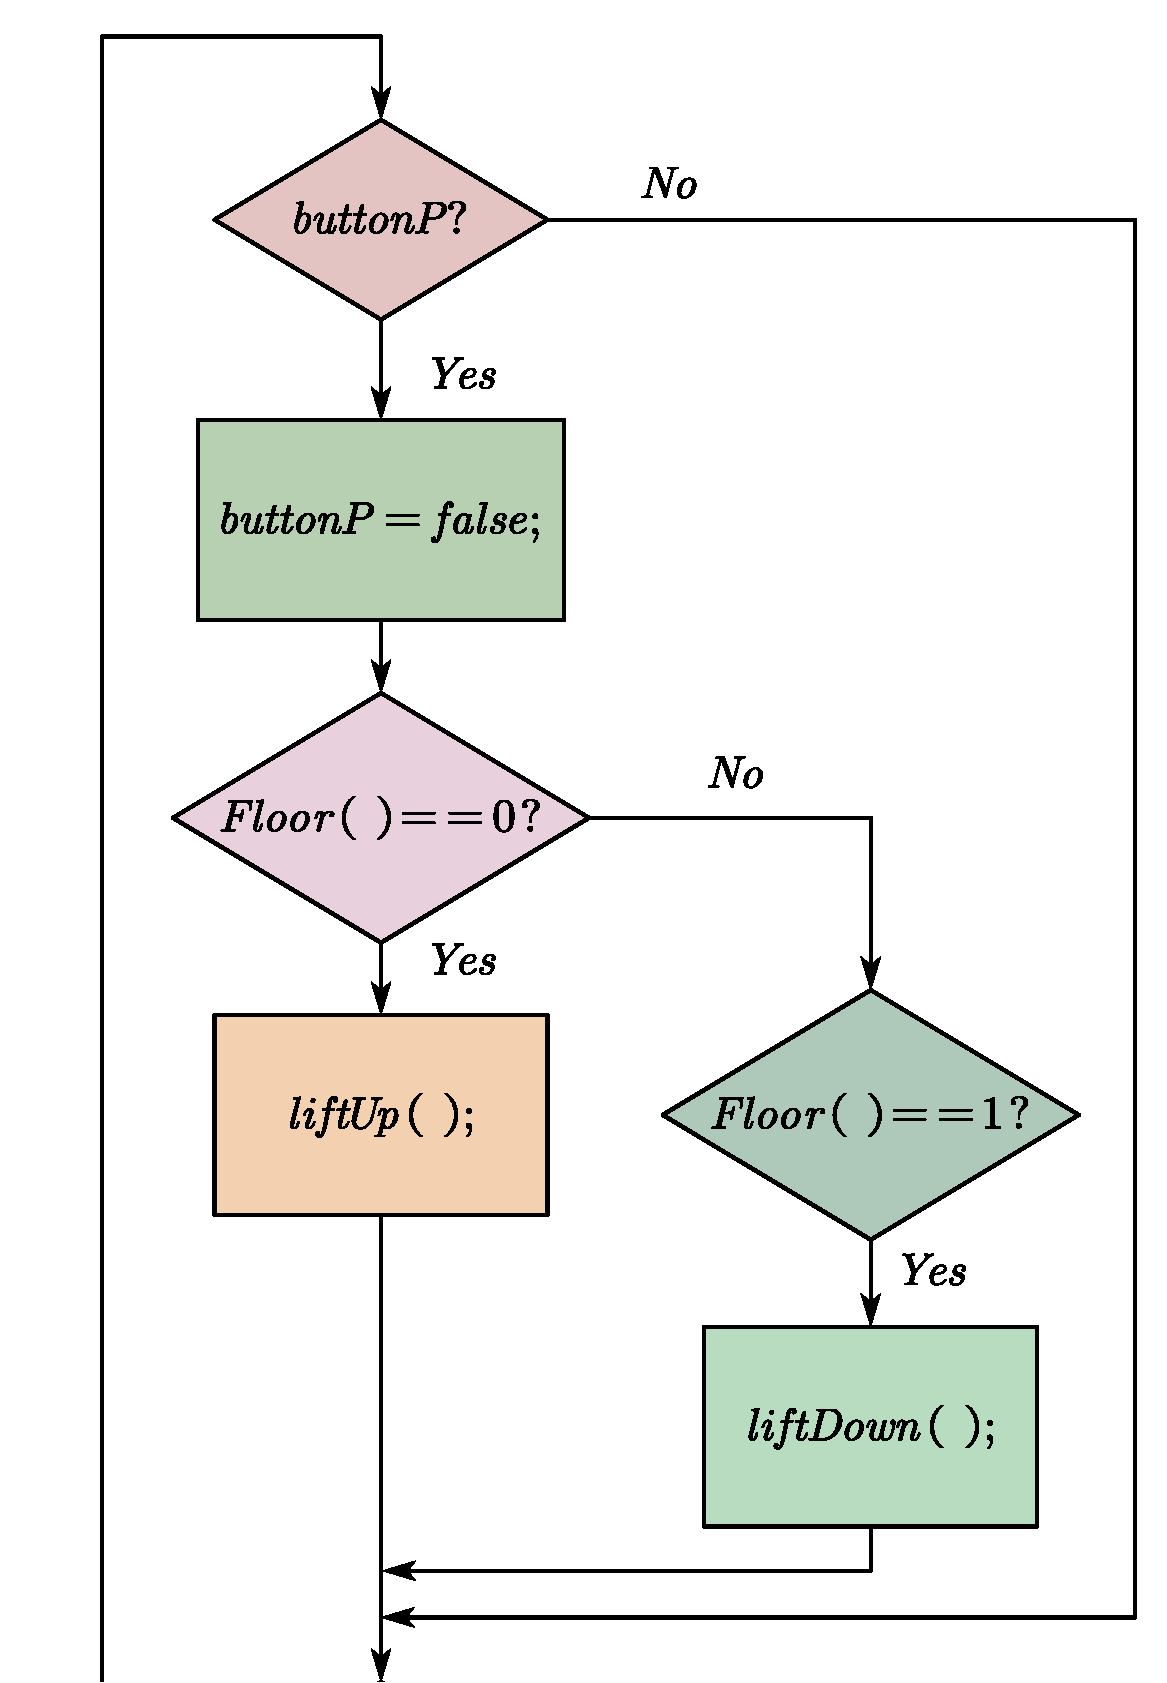
\includegraphics[width=0.5\textwidth]{Graphics/AXGLYPH_PDF/while_1st.pdf}
     \caption{First part infinite loop flowchart}
     \label{fig:firstFlow}
     \end{figure}
\end{column}
\end{columns}
\end{frame}

\begin{frame}{Implementation III}
\begin{columns}
\begin{column}{0.5\textwidth}
   Next, the loop checks if the \textbf{\textit{timer5endFlag}} is set. As the name states, this flag is set when the 5 seconds timer generates an interrupt (TIM3, as we will see later). If it is set, it calls the function \textit{liftStop()}, which re-enables the EXTI0 and the TIM3 interrupts, turns off the orange and red LEDs, updates the current floor value depending on the direction of the lift's movement, and, finally, opens the doors. As we mentioned before, the system communicates the different steps via the UART.
\end{column}
\begin{column}{0.5\textwidth}  
    \begin{figure}
    \centering
     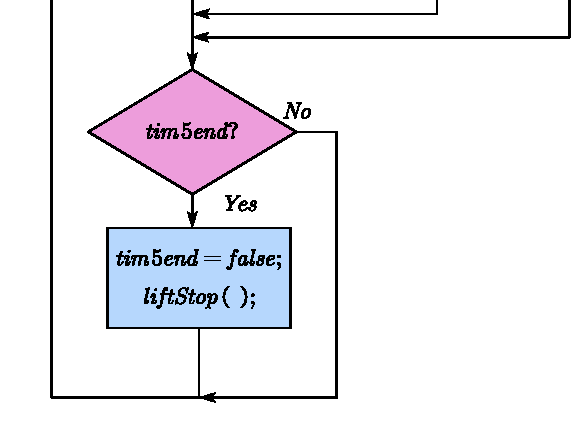
\includegraphics[width=0.5\textwidth]{Graphics/AXGLYPH_PDF/while_2nd.pdf}
     \caption{Second part infinite loop flowchart}
     \label{fig:secondFlow}
     \end{figure}
\end{column}
\end{columns}
\end{frame}




\begin{frame}{Implementation IV}
\begin{columns}
\begin{column}{0.5\textwidth}
   Regarding the interrupts, in order to reduce the time that the CPU stays inside of them, when the ISR is called, only the aforementioned flags are set. Since the structure of this project in particular is sequential, the functions that we have implemented could have been called in the callback of the ISRs themselves, but we decided not to do this because it is not good practice.
   
\end{column}
\begin{column}{0.5\textwidth}  
    \begin{figure}
    \centering
     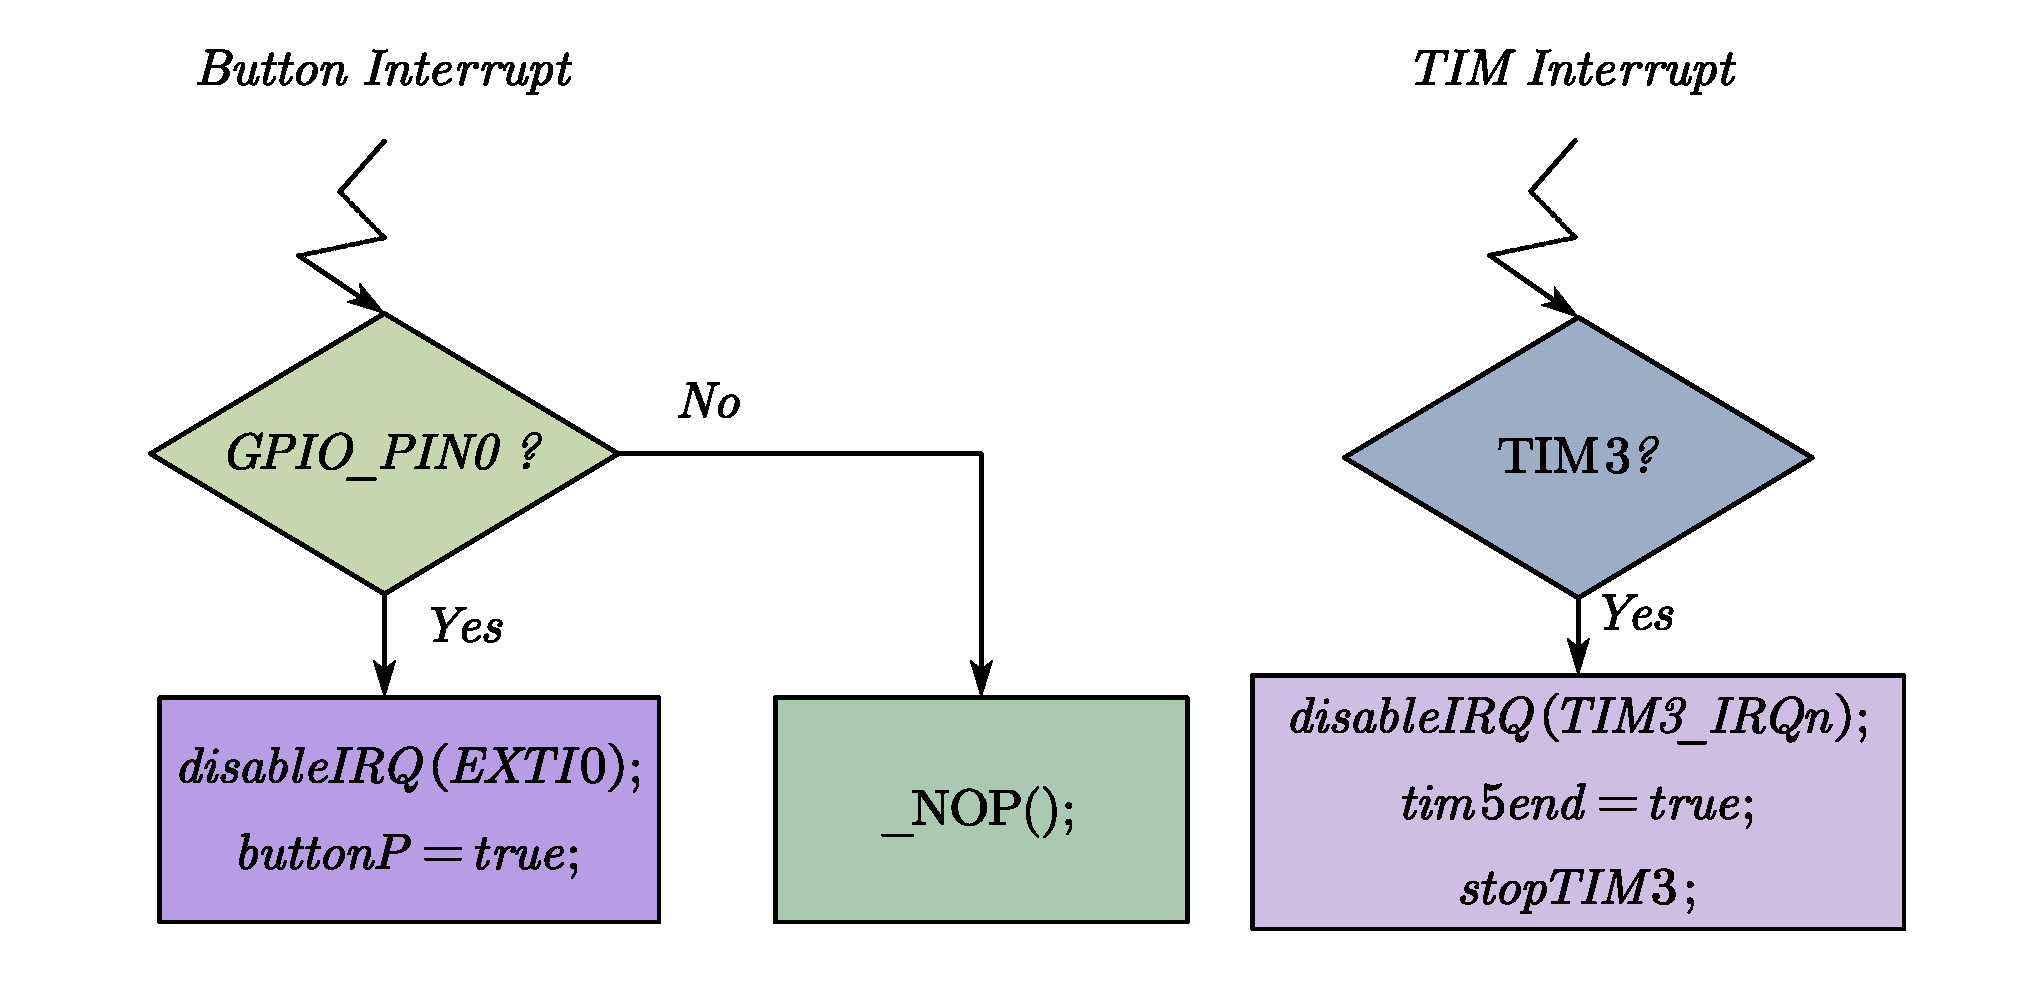
\includegraphics[width=1\textwidth]{Graphics/AXGLYPH_PDF/TIM_ISR.pdf}
     \caption{Interrupts flowchart}
     \label{fig:intFlow}
     \end{figure}
\end{column}
\end{columns}
\end{frame}

\begin{frame}{Implementation V}
This is how we have organized the set of functions shown in the subfiles. We have developed more functions but these are the most relevant ones used in \textit{lift.c}.

\begin{figure}[H]
    \centering
    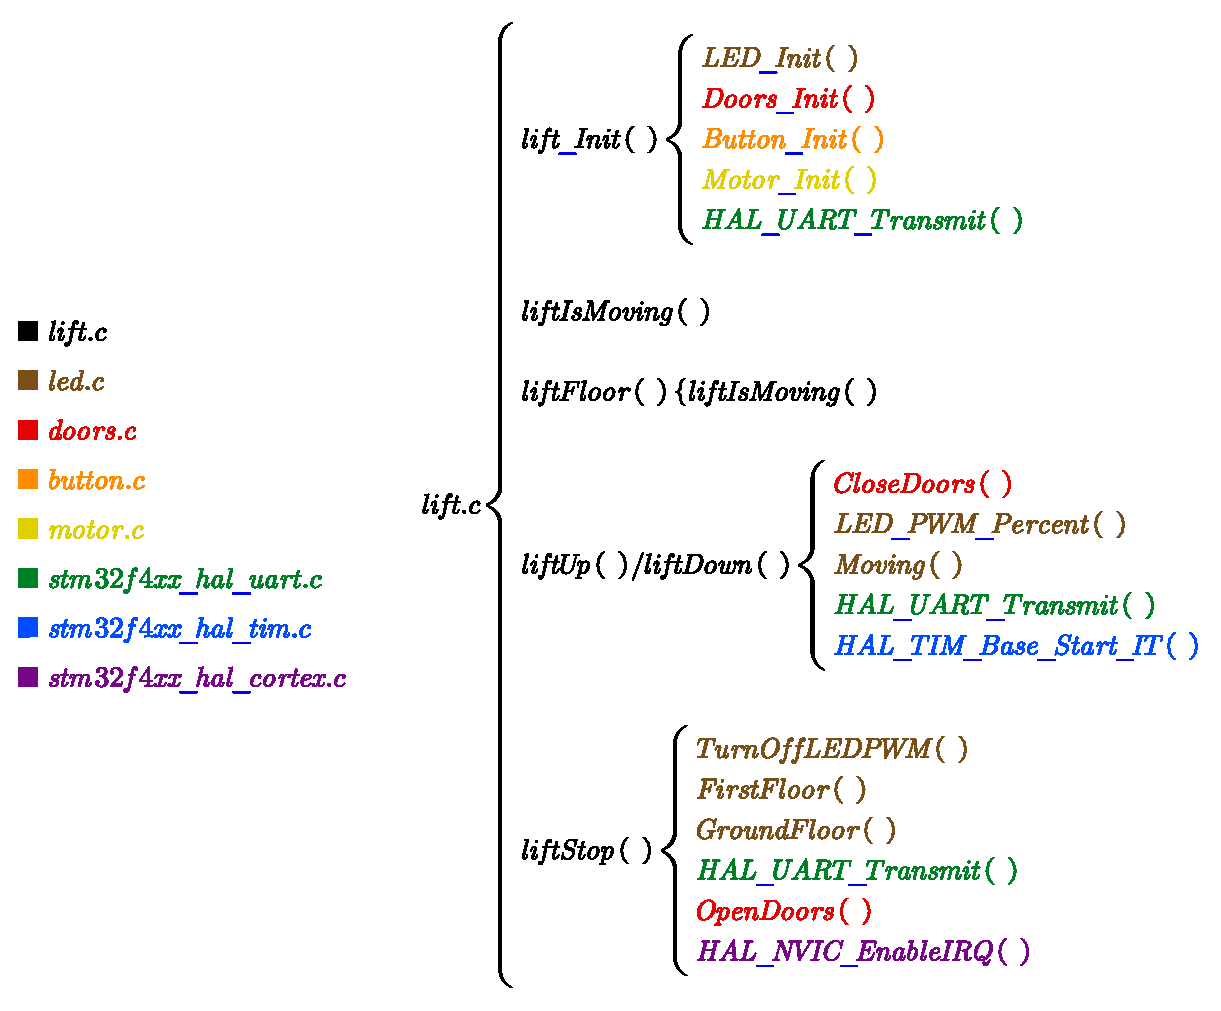
\includegraphics[width=0.45\textwidth]{Graphics/AXGLYPH_PDF/TREE.pdf}
    \caption{File dependency tree}
    \label{fig:File_management}
\end{figure}

\end{frame}

\section{Clock and peripherals configuration}
\subsection{Clocks}
\begin{frame}{Clocks}
The internal clocks were configured as stated in the lab sessions:
\begin{figure}
    \centering
    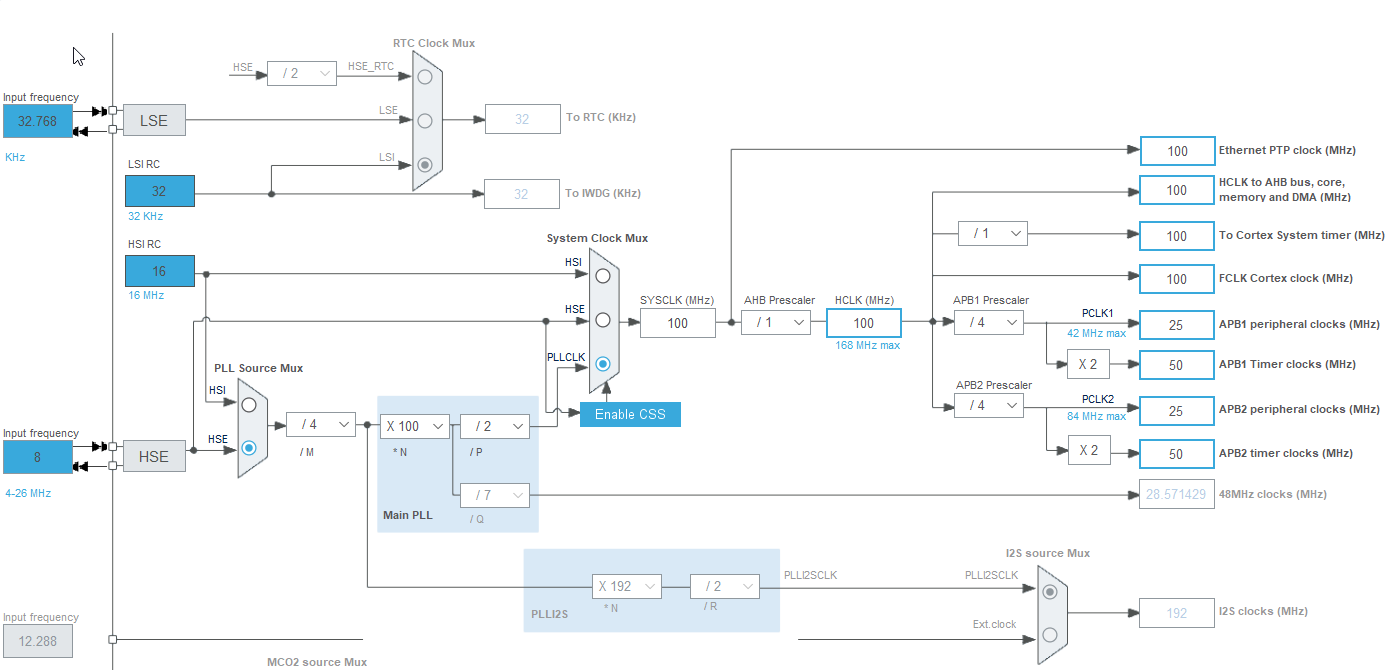
\includegraphics[width=0.75\linewidth]{Graphics/clock_conf.png}
    \caption{Internal clocks}
    \label{fig:Internal_clocks}
\end{figure}
\end{frame}

\subsection{GPIO}
\begin{frame}{GPIO}

\begin{itemize}
    \item Blue Pushbutton 
        \begin{itemize}
            \item \textbf{PA0:} GPIO\_EXTI0, no pull-up no pull-down. 
        \end{itemize}
    
    \item UART Communication
        \begin{itemize}
            \item \textbf{PA2, PA3:} USART2\_TX, USART2\_RX.
        \end{itemize}
    
    \item Stepper Motor
        \begin{itemize}
            \item \textbf{PB12, PB13, PB14, PB15:} GPIO\_Output, Push-Pull, no internal resistor, output speed low.
        \end{itemize}
    
    \item Servomotor
        \begin{itemize}
            \item \textbf{PE9:} TIM1\_CH1.
            \item \textbf{PE11:} TIM1\_CH2.
        \end{itemize}
        
    \item Floor Number LEDs
        \begin{itemize}
            \item \textbf{PD12 (Green Led), PD15 (Blue Led):} GPIO\_Output, Push-Pull, no internal resistor, output speed low.
        \end{itemize}
        
    \item State LEDs
        \begin{itemize}
            \item \textbf{PD13 (Orange Led):} TIM4\_CH2.
            \item \textbf{PD14 (Red Led):} TIM4\_CH3.
        \end{itemize}
        
\end{itemize}
\end{frame}

\begin{frame}{GPIO}

In order to fulfill the project requirements, this is the final configuration of CubeMX:

\begin{figure}
    \centering
    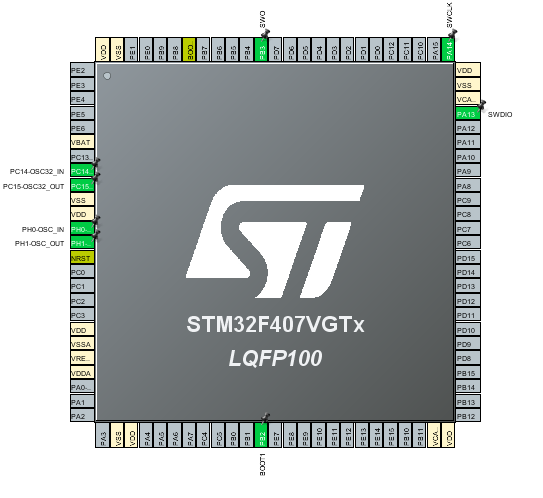
\includegraphics[width=0.25\linewidth]{Graphics/pinout_conf_nada.png}
    \caption{STM32F407 final pin configuration in CubeMX}
    \label{fig:pin_todo}
\end{figure}

The only auto-generated file that remains in the final project is the GPIO configuration file, \textit{GPIO.c}, as it cannot be removed. It is important to remark that lines 65 and 66 of the file \textit{stm32f4xx\_hal\_conf.h} must be uncommented after the generation of the code in CubeMX in order for the timers and UART to work. 
\end{frame}

\subsection{Timers}
\begin{frame}{Timers}

\vspace{-0.7 cm}

\begin{align*}

        \mathrm{TIM1} (\mathrm{T} = 20\;\mathrm{ms)} \rightarrow \left\{ \begin{aligned}
	        \mathrm{TIM1 \; CLK} &= \,\, \dfrac{50\;\mathrm{MHz}}{\mathrm{Presc}} \, = \,\, \dfrac{50\;\mathrm{MHz}}{500} = 100\;\mathrm{kHz}\\[\bigskipamount]
	        \,\, \mathrm{Counter \; period} &= \left( \left( \mathrm{TIM1 \; CLK}\right) \cdot \mathrm{T} -\,\,1 \right) = 1999\\
        \end{aligned} \right. \\[\bigskipamount]

        \hspace{0.35cm} \mathrm{TIM3} (\mathrm{T} = 5\;\mathrm{s)} \rightarrow \left\{ \begin{aligned}
	        \mathrm{TIM3 \; CLK} &= \,\, \dfrac{50\;\mathrm{MHz}}{\mathrm{Presc}} \, = \,\, \dfrac{50\;\mathrm{MHz}}{50000} = 1\;\mathrm{kHz}\\[\bigskipamount]
	        \,\, \mathrm{Counter \; period} &= \left( \left( \mathrm{TIM3 \; CLK} \right) \cdot \mathrm{T} -\,\,1 \right) = 4999\\
        \end{aligned} \right. \\[\bigskipamount]
  
        \hspace{0.35cm} \mathrm{TIM4} (\mathrm{T} = 1\;\mathrm{s)} \rightarrow \left\{ \begin{aligned}
	        \mathrm{TIM4 \; CLK} &= \,\, \dfrac{50\;\mathrm{MHz}}{\mathrm{Presc}} \, = \,\, \dfrac{50\;\mathrm{MHz}}{5000} = 10\;\mathrm{kHz}\\[\bigskipamount]
	        \,\, \mathrm{Counter \; period} &= \left( \left( \mathrm{TIM4 \; CLK} \right) \cdot \mathrm{T} -\,\,1 \right) = 999\\
        \end{aligned} \right. \\[\bigskipamount]
    
\end{align*} 
\end{frame}

\subsection{USART}
\begin{frame}{USART}
    The USART pins are the ones presented in previous slides. The configuration is performed in order to have an asynchronous communication (no external clock needed), with a baud rate (bits/sec) of 9600, which is a common value for these type of communications.
\end{frame}

\section{Hardware}
\subsection{LEDs}
\begin{frame}[fragile]{LEDs}
    The green and the blue LEDs are controlled by a set of HAL functions. In order to control the orange and red LEDs, the function \textbf{\textit{LED\_PWM\_Percent()}} was implemented.
    
    \inputCcode{Code/LED_PWM_Percent.c}
\end{frame}

\subsection{Servo motors}
\begin{frame}[fragile]{Servo motors}
    Two servo motors are connected to PWM pins PE9 and PE11. Their duty cycle is calculated as a function of the required angle in the function \textbf{\textit{Servo\_PWM\_Angle()}}. The pulse duration was obtained from the datasheet~\autocite{Parallax} provided by the manufacturer.
    
    \inputCcode{Code/Servo_PWM_Angle.c}
    
\end{frame}

\subsection{Stepper motor}
\begin{frame}[fragile]{Stepper motors}
    The stepper motor is controlled using a LUT in half-step mode (8 possible steps). We have taken advantage of the SysTick interrupt (every ms) to increment/decrement the LUT index depending on the destination floor, and to write its contents to the 4 pins that control the stepper motor driver.
    \inputCcode{Code/SysTick_Handler.c}
\end{frame}


\subsection{UART communication}
\begin{frame}[fragile]{UART communication}
    Since the UART configuration was previously defined, in order to send UART messages from the microcontroller, we have used the existing HAL function \textbf{\textit{HAL\_UART\_Transmit()}}. 
    \inputCcode{Code/uart.c}
\end{frame}

\section{Extra information}
\begin{frame}{Extra information}

    This project is available on \href{https://github.com/anacalo24/MicroProject}{Github}, as well as the necessary documents to reproduce the operation of the system. In addition, other documents such as this presentation are also accessible. We encourage you to read the project documentation we created with the help of \textit{Doxygen}, on \href{}{this link} you can find the explanation of this presentation and a video showcasing the developed application in real time.

    
\end{frame}


\begin{frame}[fragile]{Conclusion}
    \begin{center}
    \textit{\textbf{\LARGE Thank you!}}
    \end{center}
\end{frame}



\begin{frame}{References}
    \printbibliography[heading=none]
\end{frame}


\end{document}